\section{Overall approach}%
\label{approach}
Our goal is to enable private and reliable file exchange between users 
participating in the system, by using their respective devices only.
When Alice and Bob, two users of our system, want to exchange a file \(f\) 
through \name, they start by sharing some information out-of-band, comparable 
to links for sharing a file in the Cloud.
More precisely, they exchange metadata on \(f\), encryption keys, and
some single-use reply mix-headers.
They use these reply headers to transfer the file contents of \(f\) over a 
network of unreliable nodes while also achieving privacy.

After the initial, out-of-band setup, file transfer happens along
onion routes with the following features:\\
\begin{description}
  \item[Stateless] There is no circuit creation.
    The protocol is stateless up to remembering previously seen packets to 
    prevent replay attacks.
    (There is no relation between packets.)

  \item[Probabilistic] Instead of source routes with one node per onion layer, 
    each layer consists of a set of nodes and although the source route still 
    determines the sequence of layers, the actual node used for the next hop of 
    forwarding is selected from the set in an ad-hoc way\daniel{%
      What is \enquote{ad-hoc way}?}, resulting in a source-bounded random 
    walk.

  \item[Onion Routing] Put simply, in onion routing, the sender creates a 
    source route and encapsulates the payload and next-hop information in 
    layers (by encryption), that are \emph{peeled} (decrypted) one by one along 
    the route. By virtue of these layers, the forwarding nodes on the route do 
    not know where on the route they are and thus whether they have received a 
    packet directly from the sender or some other intermediate node. We base 
    our format for layering and peeling on the \ac{Sphinx} mix-header format, 
    which we extend to allow for sets of nodes in each layer.
\end{description}

% \begin{description}
% \item [Stateless.] There is no mandatory circuit creation, the file transfer can be
%   done in a stateless way. 
% \item [Predictive.] The choice of nodes included in the onion routing
%   layers is based on a predictive model for availability, disseminated
%   by an overlay and queried by random peer sampling.
% \item [Probabilistic.] Instead of source routes with one node per onion layer, each
%   layer consists of a set of nodes and although the source route still
%   determines the sequence of layers, the actual node used for the next
%   hop of forwarding is selected from the set in an ad-hoc way,
%   resulting in a source-bounded random walk.
% \item[Onion Routing.] Put simply, in onion routing, the sender creates
%   a source route and 
%   encapsulates the payload and next-hop information in layers (by
%   encryption), that are \emph{peeled} (decrypted) one by one along the
%   route. By virtue of these layers, the forwarding nodes on the
%   route do not know where on the route they are and thus whether they
%   have received a packet directly from the sender or some other
%   intermediate node. We base our format for layering and peeling on
%   \ac{Sphinx}, with some modification to allow for the
%   changes above, described in \cref{Sphinxes}.
% \end{description} 

%\subsection{Taxonomy of anonymous communication protocols}

To present the different parts of \name in detail, 
we align the presentation of the system with the taxonomy of 
\textcite{RoutingSurveyAnonymousProtocols}.
They characterize anonymous communication protocols using the following 
categories: (i) \textit{network structure}%~\ding{168}
, (ii) \textit{routing information}%~\ding{169}
, (iii) \textit{communication model}%~\ding{170}
, and (iv) \textit{performance}%~\ding{171}
~(see~\cite[Table~1]{RoutingSurveyAnonymousProtocols}).

% \begin{description}
%   \item[Network structure.]
%     It describes the characteristics of the network nodes, the connections between 
%     them and the underlying topology.
%     The subcategories are
%     \begin{enumerate*}
%       \item network topology,
%       \item connection type (direction, synchronization),
%       \item symmetry (node roles, node topology for routing, decentralization);
%     \end{enumerate*}

%   \item[Routing information.]
%     It describes the network information available to entities deciding on 
%     the route of an anonymous file exchange.
%     The subcategories are
%     \begin{enumerate*}
%       \item network view necessary for making routing decisions,
%       \item triggers for routing information updates;
%     \end{enumerate*}

%   \item[Communication model.]
%    It describes the entities that make the routing decisions and how they 
%     make these decisions.
%     The subcategories are
%     \begin{enumerate*}
%       \item routing type (who selects nodes per route),
%       \item scheduling (traffic prioritization),
%       \item node selection (determinism, selection set, selection probability);
%     \end{enumerate*}

%   \item[Performance.]
%     It describes things like latency and communication mode.
%     The subcategories are
%     \begin{enumerate*}
%       \item protocol latency,
%       \item communication mode (connection- or message-based).
%     \end{enumerate*}
% \end{description}

As depicted in \cref{fig:outline}, \ac{SPORES} relies on a probabilistic onion 
routing protocol (\ac{SPOR}). \Ac{SPOR} in turn combines a set-based mix-header 
format (\Sphinxes) together with a node selection protocol.
%% Particularly, \sphinxes (\cref{Sphinxes}), is an adaptation of the 
%% \sonja{do we apply all categories here?} \ac{Sphinx} mix-header format.
%% This means that we inherit some properties from \ac{Sphinx} and due to being only a 
%% header format, it only imposes some restrictions in the above categories.
\Sphinxes (Figure~\ref{fig:outline} \ding{202}, \cref{Sphinxes}) provides, just 
as \ac{Sphinx}, unidirectional (network structure), message-based (performance) 
communication.
But unlike \ac{Sphinx}, \Sphinxes is a hybrid: source-hop-by-hop routed, 
essentially a source-bounded random walk (communication model).
\Sphinxes relies on a flat routing-topology (network structure) with fair 
scheduling (communication model) --- as all packets are indistinguishable they 
must be processed on a first-in-first-out basis.
\Sphinxes also introduces some probability to the node selection, but this is 
only a probabilistic selection among already selected nodes and only 
interesting against passive adversaries (an active adversary can learn the 
entire set just as she can learn the single node constituting a layer of a
secure onion-routing scheme, this does not endanger the security
properties~\cite{CLOnionRouting}).

\begin{figure}[t]
  \centering
  \def\svgwidth{0.8\columnwidth}
  %  \import{figures/}{outline_figure_only.pdf_tex}
    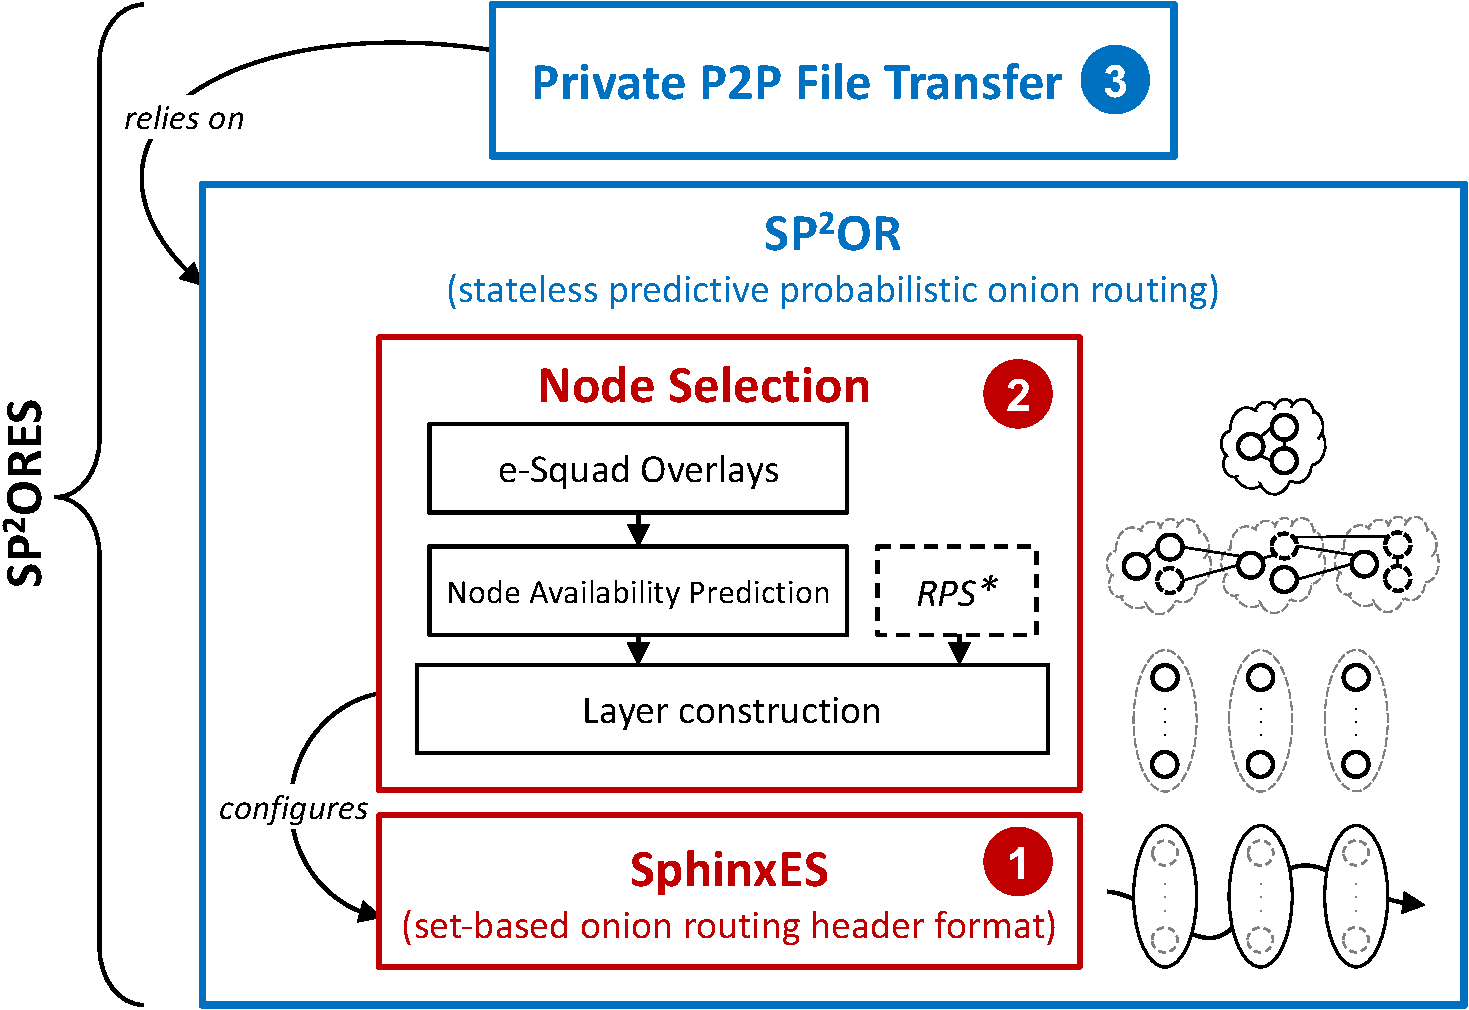
\includegraphics[width=\columnwidth]{figures/OverviewSPORES_cropped}
    \caption{%
      Architectural overview of the \ac{SPORES} private file sharing service.
      \daniel{This figure must be updated.}
    }
    \label{fig:outline}
\end{figure}

\Sphinxes does \emph{not} introduce any restrictions on whether the network 
topology must be fully connected or not, be asynchronous (as in Tor) or 
synchronous (as in mix-nets), whether node selection must be uniformly random 
or not.
Just as \ac{Sphinx}, it can be used in many different settings.

Further, the \ac{SPOR} protocol (\cref{design}) adds node selection on top of \Sphinxes.
The \ac{SPOR} protocol (Figure~\ref{fig:outline} \ding{203})  assumes a source of random nodes, \eg through 
\ac{RPS}~\cite[\eg][]{BrahmsRPS} or \iac{DHT} based 
scheme~\cite[\eg][]{Octopus}.
The choice of this source of random nodes affects the network view (routing 
information) of each node, as well as how decentralized the scheme becomes and 
whether the network topology is fully, mostly or partly connected (network 
structure).

Each node must be associated with a public key and some prediction function.
\Ac{SPOR} selects nodes for a route uniformly randomly and uses the prediction 
function to optimize the properties of the entire route, \ie across layers.
As \ac{SPOR} is designed, it selects nodes uniformly among all the nodes 
(communication model, node selection) that the source of random nodes provides.
Thus, ultimately, these also depends on the source of random nodes.

Finally, we introduce the complete \ac{SPORES} protocol that allows 
transferring larger messages by fragmentation and reassembly across the devices 
in the \squad  (Figure~\ref{fig:outline} \ding{204}).
